\documentclass{article}
% Chinese
% \documentclass[UTF8, nofonts, mathptmx, 12pt, onecolumn]{article}
% \usepackage{xeCJK}
% \setCJKmainfont{SimSun}
\usepackage{amsmath}
\usepackage{amsfonts}
\usepackage{amssymb}
\usepackage{wasysym}
% \usepackage{ctex}
\usepackage{graphicx}
\usepackage{float}
\usepackage{geometry}
\geometry{a4paper,scale=0.8}
\usepackage{caption}
\usepackage{subcaption}
% \newcommand{\oiint}{\mathop{{\int\!\!\!\!\!\int}\mkern-21mu \bigcirc} {}}
\newcommand*{\dif}{\mathop{}\!\mathrm{d}}
\newcommand*{\md}{\mathop{}\!\mathrm{d}}
\newcommand*{\me}{\mathrm{e}}

% \usepackage{parskip}
% \setlength{\parindent}{0cm}

\usepackage{bm}
\let\Oldmathbf\mathbf
\renewcommand{\mathbf}[1]{\boldsymbol{\Oldmathbf{#1}}}
\let\eqnarray\align

\author{Xiping Hu}
\usepackage{authblk}
\author{Xiping Hu}
\affil{https://hxp.plus/}
\title{Homework for Chapter 1}

\begin{document}
\maketitle

\begin{figure}[H]
  \centering
  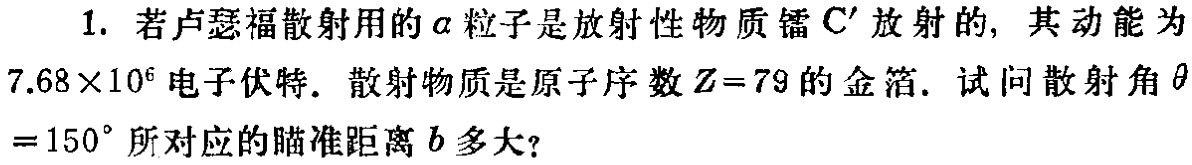
\includegraphics[width=\linewidth]{figures/Problem1}
  \label{fig:}
\end{figure}

From Rutherford's scattering

\begin{equation*}
  \begin{aligned}
    C = \dfrac{Z e^2}{2 \pi \varepsilon_0} 
  \end{aligned}
\end{equation*}

\begin{equation*}
  \begin{aligned}
    \cot \dfrac{\theta}{2} = \dfrac{2 E_0 b}{C}  
  \end{aligned}
\end{equation*}

So that

\begin{equation*}
  \begin{aligned}
    b = \dfrac{1}{2 E_0}  \dfrac{Z e^2}{2 \pi \varepsilon_0} \cot \dfrac{\theta}{2} = 3.97 \times 10^{-15} \  \mathrm{m}
  \end{aligned}
\end{equation*}

\begin{figure}[H]
  \centering
  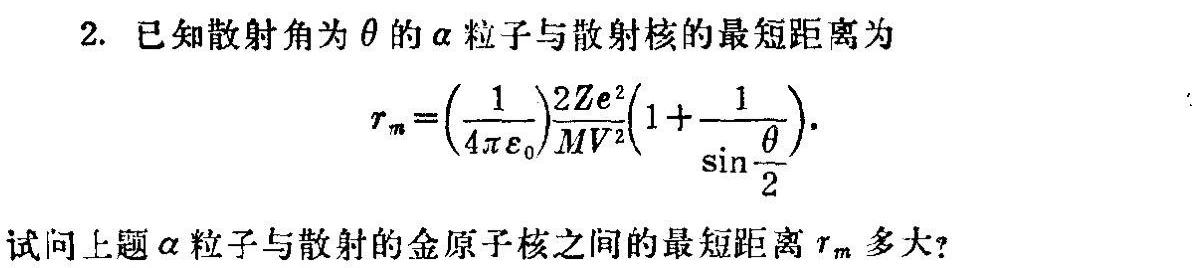
\includegraphics[width=\linewidth]{figures/Problem2}
  \label{fig:}
\end{figure}

\begin{equation*}
  \begin{aligned}
    r_m = \left( \dfrac{1}{4 \pi \varepsilon_0} \right) \dfrac{2Ze^2}{2 E_0} \left( 1 + \dfrac{1}{\sin \dfrac{\theta}{2} }  \right) = 3.01 \times 10^{-14} \  \mathrm{m}
  \end{aligned}
\end{equation*}

\begin{figure}[H]
  \centering
  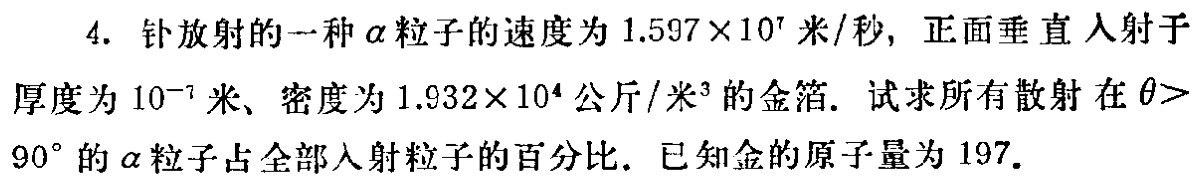
\includegraphics[width=\linewidth]{figures/Problem4}
  \label{fig:}
\end{figure}

What we have already known is:

\begin{equation*}
  \begin{aligned}
    b = \dfrac{1}{2 E_0}  \dfrac{Z e^2}{2 \pi \varepsilon_0} \cot \dfrac{\theta}{2}
  \end{aligned}
\end{equation*}

We take the derivative

\begin{equation*}
  \begin{aligned}
    \md b = \dfrac{1}{2 E_0}  \dfrac{Z e^2}{2 \pi \varepsilon_0} \dfrac{\cos \dfrac{\theta}{2} }{\sin^3 \dfrac{\theta}{2} } \md \theta
  \end{aligned}
\end{equation*}

\begin{figure}[H]
  \centering
  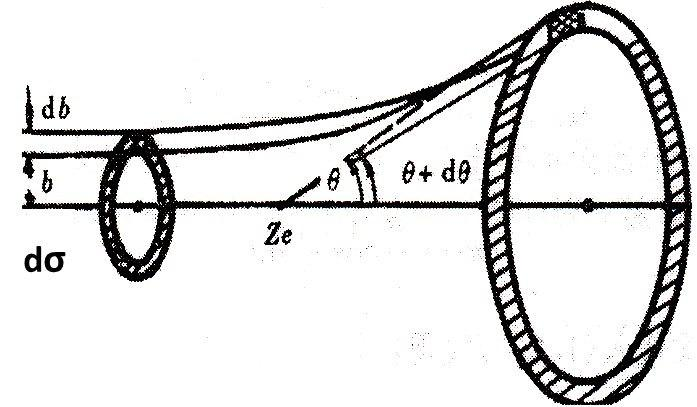
\includegraphics[width=0.5\linewidth]{figures/Rutherford-1}
  \label{fig:}
\end{figure}

\begin{equation*}
  \begin{aligned}
    \dfrac{\md n}{n} = N t \md \sigma = N t \cdot 2 \pi b \md b = \dfrac{\rho N_A t}{Z} \pi \left( \dfrac{1}{4 \pi \varepsilon_0}  \right)^2 \left( \dfrac{2 Z e^2}{m v^2}  \right)^2 \dfrac{\cos \dfrac{\theta}{2} }{\sin^3 \dfrac{\theta}{2} } \md \theta
  \end{aligned}
\end{equation*}

\begin{equation*}
  \begin{aligned}
    \dfrac{\Delta n}{n} =  \dfrac{\rho N_A t}{Z} \pi \left( \dfrac{1}{4 \pi \varepsilon_0}  \right)^2 \left( \dfrac{2 Z e^2}{m v^2}  \right)^2 \int_{\frac{\pi}{2} }^{\pi} \dfrac{\cos \dfrac{\theta}{2} }{\sin^3 \dfrac{\theta}{2} } \md \theta = 8.5 \times 10^{-6}
  \end{aligned}
\end{equation*}

\begin{figure}[H]
  \centering
  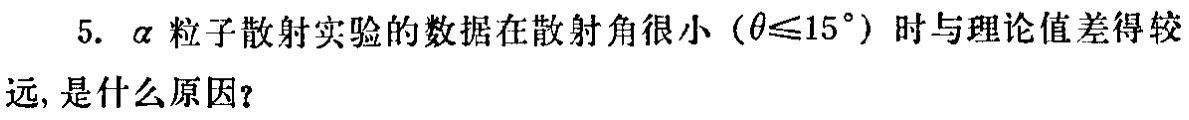
\includegraphics[width=\linewidth]{figures/Problem5}
  \label{fig:}
\end{figure}

This is partly because that we assumed there was only one layer of gold atoms in gold foil, and the alpha particles would only be scattered once. But in fact, there are several layers of gold atoms. For small angle scattering results, since the result was accumulated by some small angle scatterings, each cannot be ignored and contributes to a large proportion of error.

\end{document}